\pagebreak
\subsection{Friction test} %\label{put a label here and uncomment}
\textbf{Name: Group 510}\\
\textbf{Date: 28/10 - 2015}

\subsubsection{Purpose}
The purpose of the test is to find the total friction, $B$, of the vehicle.

\subsubsection{Setup}
\begin{figure}[H]
  \centering
	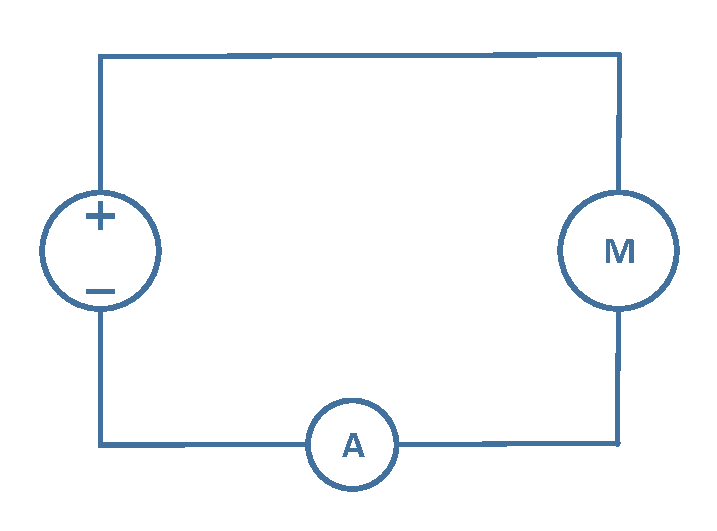
\includegraphics[scale=0.5]{figures/FrictionTest.pdf}
	\caption{A diagram of the test setup}
\end{figure}

\subsubsection{List of Equipment}

\begin{table}[H]
\begin{tabular}{|l|l|p{4cm}|}
\hline%------------------------------------------------------------------------------------
  \textbf{Instrument}                        &  \textbf{AAU-no.}  &  \textbf{Type}       \\
\hline%------------------------------------------------------------------------------------
  Multimeter                               &  60764             &  fluke 189 true RMS    \\
\hline%------------------------------------------------------------------------------------
  Power Supply ($0 - 32$ V) ($0 - 10$ A)     &  77075             &  Ea - ps 7032 - 100  \\
\hline%------------------------------------------------------------------------------------
  Treadmill                         &  75483             &  Rodby            \\
\hline%------------------------------------------------------------------------------------
\end{tabular}
\end{table}

\subsubsection{Procedure}

\begin{enumerate}
  \item Connect the power supply's power channel to the motor and the ground channel to the multimeter.
  \item Place the vehicle in the middle of the treadmill.
  \item Set the power channel to under $4$ amperes, the vehicle is not running, but ready to run when the power supply is set above $4$ amperes later. 
  \item Activated the treadmill to run at the required speed, and at the same time correct the power supply so the vehicle receives more than $4$ amperes and thereby making it move.
  \item Correct the speed of the vehicle with the power supply until the vehicle has the same velocity as the treadmill.
  \item Read the current on the multimeter.
  \item Repeat the process with different velocities.
\end{enumerate}

\subsubsection{Results}

